\documentclass[]{article}
\usepackage{amsmath}\usepackage{amsfonts}
\usepackage[margin=1in,footskip=0.25in]{geometry}
\usepackage{mathtools}
\usepackage{hyperref}
\hypersetup{
    colorlinks=true,
    linkcolor=blue,
    filecolor=magenta,
    urlcolor=cyan,
}
\usepackage[final]{graphicx}
\usepackage{listings}
\usepackage{courier}
\lstset{basicstyle=\footnotesize\ttfamily,breaklines=true}
\newcommand{\indep}{\perp \!\!\! \perp}
% \usepackage{wrapfig}
\graphicspath{{.}}
% \usepackage{fancyvrb}

%%
%% Julia definition (c) 2014 Jubobs
%%
\usepackage[T1]{fontenc}
\usepackage{beramono}
\usepackage[usenames,dvipsnames]{xcolor}
\lstdefinelanguage{Julia}%
  {morekeywords={abstract,break,case,catch,const,continue,do,else,elseif,%
      end,export,false,for,function,immutable,import,importall,if,in,%
      macro,module,otherwise,quote,return,switch,true,try,type,typealias,%
      using,while},%
   sensitive=true,%
   alsoother={$},%
   morecomment=[l]\#,%
   morecomment=[n]{\#=}{=\#},%
   morestring=[s]{"}{"},%
   morestring=[m]{'}{'},%
}[keywords,comments,strings]%

\lstset{%
    language         = Julia,
    basicstyle       = \ttfamily,
    keywordstyle     = \bfseries\color{blue},
    stringstyle      = \color{magenta},
    commentstyle     = \color{ForestGreen},
    showstringspaces = false,
}


\begin{document}
\begin{center}
    Name: Hongda Li 
    \\
    AMATH 585 WINTER 2022 HW3
\end{center}
\section*{Problem 1}
    \subsection*{Problem 1 Code}
        \begin{lstlisting}
"""
A Struct for storing all the relevant paramters for the 
nont linear pendulum problems
"""
mutable struct PendulumProblem
    # primary paramters 
    m           # M + 1 is the number of grid points including the boundary 
                # conditions. 
    alpha       # boundary condition when t = 0. 
    beta        # boundary condition when t = T. 
    # second dary parameters
    h           # time domain division 

    # running parameters
    theta_k     # the kth guess 

    function PendulumProblem(m, alpha, beta, T, theta0)
        this = new()
        this.m = m
        this.alpha = alpha
        this.beta = beta
        this.h = T/(m + 1)
        this.theta_k = theta0
        return this 
    end

end


"""
    Get the jacobian matrix given a trajector over the time interval. 
"""
function EvalJacobiAt(this::PendulumProblem, theta) 
    @assert length(theta) == this.m "The given trajectory must agree with"*
    " the problem parameters, more precisely, the grid discretization."*
    "We expect shape ($(this.m),) for function: EvalJacobiAt,"*
    " but we got: $(size(theta)). "
    diagonals = zeros(this.m)
    @. diagonals = -2/this.h^2 + cos(theta)
    subdiagonals = fill(1/this.h^2, this.m)
    return SymTridiagonal(diagonals, subdiagonals)
end

function EvalJacobiAt(this::PendulumProblem)
    return EvalJacobiAt(this, this.theta_k)
end


"""
    Get the value of the non-linear finite diff given the trajactory of the 
    pendulum. 
"""
function EvalAt(this::PendulumProblem, theta)
    h = this.h
    v = zeros(this.m)
    
    # Boundary for t = 0, alpha. 
    v[1] = (this.alpha - 2*theta[1] + theta[2])/h^2 + sin(theta[1])
    
    # Interior 
    for i in 2:this.m - 1
        v[i] = (theta[i - 1] - 2*theta[i] + theta[i + 1])/h^2 + sin(theta[i])
    end
    
    # Boundary for t = T, beta. 
    v[end] = (theta[end - 1] - 2*theta[end] + this.beta)/h^2 + sin(theta[end])
    return v
end



"""
Evalute the pendulum problem at the most recent guesses from the newton's 
iteration. 
"""
function EvalAt(this::PendulumProblem)
    return EvalAt(this::PendulumProblem, this.theta_k)
end



"""
    Performs one step of newton iterations based on the initial conditions given
    for the construction of the problem instance. 
"""
function (this::PendulumProblem)()
    theta_k = this.theta_k - 
        EvalJacobiAt(this, this.theta_k)\EvalAt(this, this.theta_k)
    this.theta_k = theta_k
    return copy(this.theta_k)
end


"""
    Solve this given all the parameters needed for the Newton's Method for 
    Iterations. 
"""
function SolveSystemFor(m, alpha, beta, T, initial_guess)
    t = collect(LinRange(0, T, m + 2)[2:end - 1])
    theta0 = nothing
    if isa(initial_guess, Function)
        theta0 = initial_guess.(t)
    else
        theta0 = initial_guess
    end
    problem = PendulumProblem(m, alpha, beta, T, theta0)
    trajectories = Vector{Vector}()
    push!(trajectories, theta0)
    
    for i in 1:200
        push!(trajectories, problem())
        if norm(trajectories[end] - trajectories[end - 1], Inf) < 1e-8
            break
        end
    end
    for v in trajectories
        push!(v, beta)
        pushfirst!(v, alpha)
    end
    return vcat(0, t, T), trajectories
end


### ----------------------------------------------------------------------------

using LinearAlgebra, Plots

function Problem1A()
    m = 64
    alpha = 0.7
    beta = 0.7
    T = 2*pi 
    t = collect(LinRange(0, T, m + 2)[2:end - 1])
    theta0 = @. sin(2t) + 0.7
    problem = PendulumProblem(m, alpha, beta, T, theta0)
    trajectories = Vector()
    push!(trajectories, theta0)
    for i in 1:40
        push!(trajectories, problem())
        if norm(trajectories[end] - trajectories[end - 1], Inf) < 1e-8
            break
        end
    end

    fig = plot(t, trajectories[1], label="initial guess", title="Problem 1 (a)")
    plot!(t, trajectories[end], label = "conveged")
    xlabel!(fig, "t")
    ylabel!(fig, "theta")
    savefig(fig, "problem1(a).png")
    return 
end

Problem1A();

function Problem1B()
    m = 127
    T = 10
    alpha = 0
    beta = 0
    f(t) = 2.8sin((2pi*t)/20)
    t, trajectories = SolveSystemFor(m, alpha, beta, T, f)

    # Boopstrap Boundary Conditions. 
    for epsilon in LinRange(0, 0.7, 10)
        t, trajectories = SolveSystemFor(
            m, epsilon, epsilon, T, trajectories[end][2:end-1])
    end
    
    # Bootstrap time interval.
    for T in LinRange(10, 20, 20)
        t, trajectories = SolveSystemFor(
            m, 0.7, 0.7, T, trajectories[end][2:end-1])
    end

    fig = plot(
                t, 
                trajectories[end], 
                ylim=(0, 1.1pi), 
                xlim=(t[1], t[end]), 
                title="converged solution"
            ) 
    display(fig)
    xlabel!(fig, "t")
    ylabel!(fig, "theta")
    savefig(fig, "problem1(b).png")
return end

Problem1B()        
        \end{lstlisting}
    \subsection*{1(a)}
        Purely by chance, I found another solution that swing to the left more aggressively and then swing back. This is the plot together with its initial guess for it: 
        \begin{center}
            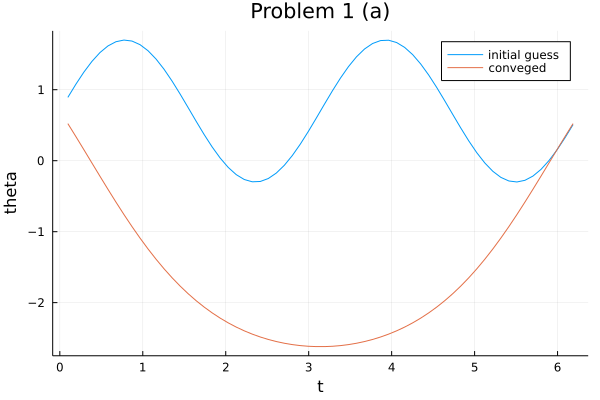
\includegraphics[width=10cm]{problem1(a).png}    
        \end{center}
        
    \subsection*{1(b)}
        \par\hspace{1.1em}
        I would like to explain the implementaions of the method before showing the plots and then the code. 
        \par
        I find the solution that first swing up, with $\theta'(t)$ be positive, for the boundary conditions $\alpha = \beta = 0$ and $T = 5$, and then I slowly changes the boundary conditions for the newton's method incrementally to $\alpha = \beta = 0.7$, each time using the solution from the newton's method from the previous parameters. 
        \par
        And then I start to increase the value of $T$ slowly and each time using the converged solution for the smaller $T$ as the initial guess for the larger value. Which made me to identify the solution for $T = 20$ that has the same characteristic as the solution found for (figure 2.5) in the textbook. 
        \begin{center}
            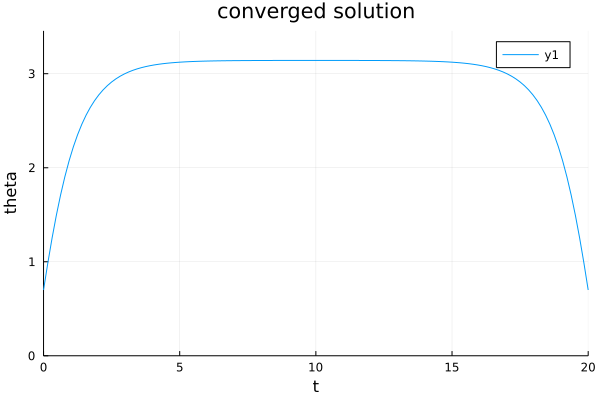
\includegraphics[width=10cm]{problem1(b).png}
        \end{center}
        Take note that, the solution swings up and then stays on the top, which is an unstable equilibruim for a long time and then drops back to the original place after $T$, as $T$ gets bigger the maximum angle of the solution ver the interval approaches $\pi$. It exhibits boundary layers problem because of the stiff derivative on the left and right boundary of the converged solution. 


    
    

\section*{Problem 2}
    Consider the problem: 
    \begin{align*}
        -u_{x x}+\left(1+x^{2}\right) u=f, \quad 0 \leq x \leq 1, \\
        u(0)=0, \quad u(1)=0 .
    \end{align*}
    Assuming uniform grid with $h = 1/(m + 1)$, where there are $m + 2$ points in total including the boundary points, then we use the finite difference scheme: 
    $$
        \frac{2 u_{i}-u_{i+1}-u_{i-1}}{h^{2}}+\left(1+x_{i}^{2}\right) u_{i}=f\left(x_{i}\right), \quad i=1, \ldots, m
    $$
    \subsection*{2(a)}
        We are going to use Gorschgorin's Theorem to place a bound on the eigenvalues for the finite difference matrix. The theorem is stated as: 
        \begin{align*}\tag{2.a.1}\label{eqn:2.a.1}
            \Lambda (A) \subseteq \bigcup_{i = 1}^n
            \left\lbrace
                x \in \mathbb{C}: | x - a_{i, i}| \le 
                \sum_{j = 1, j\neq i}^{n}| a_{i, j}|
            \right\rbrace
        \end{align*}
        Where $\Lambda(A)$ denotes the set of all eigenvalues of the matrix $A$, this is the rows of the finite difference matrix when expanded out: 
        \begin{align*}\tag{2.a.2}\label{eqn:2.a.2}
            \begin{cases}
                \frac{1}{h^2}\left(
                    (2 + h^2(1 + x_i^2))u_i - u_{i + 1} - u_{i - 1}
                \right) = f(x_i) &  i= 2, \cdots, m - 1
                \\
                \frac{1}{h^2}\left(
                    (2 + h^2(1 + x_1^2))u_1 - u_{2}
                \right)
                = f(x_i) &  i = 1
                \\
                \frac{1}{h^2}((2 + h^2(1 + x_m^2))u_m - u_{m - 1}) & i = m
            \end{cases}
        \end{align*}
        Observe that the matrix is Tridiaognla Symmetric with $-1/h^2$ as it's upper and lower sub-diagonals. 
        Let's define the radius of the disk for each row of the matrix $A$: 
        \begin{align*}\tag{2.a.3}\label{eqn:2.a.3}
            R_i (A) &= \sum_{j = 1, j\neq i}^{n}
                |a_{i, j}| = \frac{2}{h^2} \quad \forall i = 2, \cdots, m - 1
            \\
            R_1(A) &= \frac{1}{h^2}| -1| = \frac{1}{h^2} \quad i = 1
            \\
            R_m(A) &= \frac{1}{h^2}| -1| =  \frac{1}{h^2} \quad i = m
        \end{align*}
        Then we consider case by case, firstly consider: 
        \begin{align*}\tag{2.a.4}\label{eqn:2.a.4}
            \left|
                x - \frac{2}{h^2} - ( 1 + x_i^2)
            \right| 
            &\le  R_i(A) = \frac{2}{h^2} 
            \quad i = 2, \cdots, m
            \\
            \frac{-2}{h^2} &\le  
            x - \left(
                \frac{2}{h^2} + (1 + x_i^2)
            \right) \le \frac{2}{h^2}
            \\
            (1 + x_i^2) &\le  x \le \frac{4}{h^2} + (1 + x_i^2) \quad \forall i = 2, \cdots, m - 1
            \\ \underset{[1]}{\implies}
            1 + 2h^2 &\le x \le \frac{4}{h^2} + 1 + (m - 1)^2 h^2
            \\ \underset{[2]}{\implies}
            1 + 2h^2 &\le x \le \frac{4}{h^2} + 2
        \end{align*}
        \par
        [1]: I took $i = 2$ on the for the lower bound , and $i = m - 1$ for the upper bound.
        \par
        [2]: I used the substitution: $h = 1/(m + 1)$. 
        \par
        Take note that we can treat the modulus of the complex number as if it's absolute value, because the disks is centered on the real line, and the closest point to the origin will be the center offsetted by the radius of the disk. And that would be the bound on $x$. 
        \par
        And then we consider the case where $i = 1, m$ and ,look for the bound on the eigenvalues. 
        \begin{align*}\tag{2.a.5}\label{eqn:2.a.5}
            \left| 
                x - \left(
                    \frac{2}{h^2} + (1 + x_i^2)
                \right) 
            \right| &\le \frac{1}{h^2}
            \\
            \frac{1}{h^2} + (1 + x_i^2) &\le  x 
            \le     \frac{1}{h^2} + \frac{2}{h^2}
            + (1 + x_i^2)
            = \frac{3}{h^2} + (1 + x_i^2) \quad i = m, 1
            \\\implies
            \frac{1}{h^2} + (1 + (mh)^2) &\le x \le 
            \frac{3}{h^2} + (1 + (mh)^2) \quad i = m
            \\\implies 
            \frac{1}{h^2} + (1 + h^2) &\le x \le 
            \frac{3}{h^2} + (1 + h^2) \quad i = 1
        \end{align*}
        And notice that the upper bound for $x$ still seems to occur for the cause $i = 2, \cdots, m - 1$, for $h\in [0, 1]$. Therefore, the bound for the eigenvalues I would choose is: 
        \begin{align*}\tag{2.a.6}\label{eqn:2.a.6}
            \Lambda(A) &\subseteq
            \left[
                1 + (2h)^2, 
                \frac{4}{h^2} + 1 + (m -1)^2h^2
            \right]
        \end{align*}
        as the interval on the real line for the eigenvalues for the matrix $A$. 
        \par
        To justify, among all of the lower bound: $1 + 2h^2, 1/h^2 + (1 + h^2), 1/h^2 + (1 + (mh)^2)$, assuming $h \in [0, 1/2]$, the lowest is $1 + 2h^2$. Among the larger upper bound $3/h^2 + 1 + (mh)^2$ from \hyperref[eqn:2.a.5]{(2.a.5)} and the upper bound $4/h^2 + 2$ from \hyperref[eqn:2.a.4]{2.a.4}, the later is larger because $mh$ is less than one. 


    \subsection*{2(b)}
        Here we wish to show that the global error for the finite difference solution under the L2 norm is going to be as the LTE for the finite difference scheme. The LTE is simply given as: 
        \begin{align*}\tag{2.b.1}\label{eqn:2.b.1}
            \frac{2u_i - u_{i + 1} - u_{i - 1}}{h^2}
            + 
            (1 + x_i^2)u_i - f(x_i) &= \mathcal{O}(h^2) = \tau_i
        \end{align*}
        because the 2nd order central difference scheme has an error of $\mathcal{O}(h^2)$. 
        \par
        In addition, let's define the quantities $\tilde{u}$ to be the solution vector computed via the finite difference method. Let $A$ be the finite difference matrix that is paramaterized by $h$. Let $\hat{u}$ denote the exact solution vector. let $f$ denotes RHS vector, basically the function $f$ evaluated elementwise on the gridpoints we defined. $\vec{\tau}$ is the LTE vector from the finite difference scheme listed above. 
        \par
        First we consider the spectral norm inequaity. 
        Next, we plan to track the error in a way that uses the spectral norm and the relations between the L2 norm and the 2 norm. Which is just $\sqrt{h}\Vert \vec{\eta}\Vert_2 = \Vert \vec{\eta}\Vert_{L2}$
        \begin{align*}\tag{2.b.2}\label{eqn:2.b.2}
            A\hat{u} - f &= \vec{\tau} \\
            A\tilde{u} &= f
            \\
            \implies
            A\hat{u} - A\tilde{u} &= \vec{\tau}
            \\
            A(\hat{u} - \tilde{u}) &= \vec{\tau}
            \\
            \text{let: }\vec{\eta} &= \hat{u} - \tilde{u} 
            \\
            A\vec{\eta} &=\vec{\tau}
            \\
            \vec{\eta} &= A^{-1}\vec{\tau}
            \\
            \Vert \vec{\eta}\Vert_2 &\le 
            \Vert A^{-1}\Vert_2\Vert \vec{\tau}\Vert_2
        \end{align*}
        And we can figure out the upperbound spectral norm for $A^{-1}$ using the bounds we obtained for the eigenvalues for the matrix $A$. 
        \begin{align*}\tag{2.b.3}\label{eqn:2.b.3}
            \Vert A^{-1}\Vert_2^2 &= 
            \frac{
                    \lambda_{\max}(A^{-T}A^{-1})
                }{
                    \lambda_{\min}(A^{-T}A^{-1})
                }
            \\
            &= \frac{
                \lambda_{\max}((AA^T)^{-1})
            }{
                \lambda_{\min}((AA^T)^{-1})
            }
            \\
            &= 
            \frac{\lambda_{\max}((A^2)^{-1})}
            {\lambda_{\min}((A^2)^{-1})}
            \\
            &= 
            \frac{\lambda_{\min}(A^2)}{\lambda_{\max}(A^2)} = 
            \frac{\lambda_{\min}(A)^2}{\lambda_{\max}(A)^2}
            \\
            \Vert A^{-1}\Vert_2 &= 
            \frac{\lambda_{\min}(A)}{\lambda_{\max}(A)}
            \\
            \implies 
            \Vert A^{-1}\Vert_2 &\le 
            \frac{1 + (2h)^2}{\frac{4}{h^2} + 1 + (m - 1)^2h^2}
            = 
            \frac{h^2 + 4h^4}{
                4 + h^2 + (m - 1)^2h^4
            }
        \end{align*}
        Now let's consider the quantity: $\Vert \vec{\tau}\Vert_2^2$: 
        \begin{align*}\tag{2.b.4}\label{eqn:2.b.4}
            \Vert \vec{\tau}\Vert_2^2 &= 
            \sum_{j = 1}^{m} (\mathcal{O}(h^2))^2
            \\
            &= \sum_{j = 1}^{m}
            \mathcal{O}(h^4)
            \\
            &= (1/h - 1)\mathcal{O}(h^4)
            \\
            \implies &= \mathcal{O}(h^3)
            \\
            \implies
            \Vert \vec{\tau}\Vert_{L2} &= \sqrt{h}\Vert \vec{\tau}\Vert_2
            = \sqrt{h^{1/2}}\mathcal{O}(h^{3/2}) = \mathcal{O}(h^2)
        \end{align*}
        Consider again the L2 norm of the error vector $\eta$, which is given as: 
        \begin{align*}\tag{2.b.5}\label{eqn:2.b.5}
            \Vert \vec{\eta}\Vert_2 &\le 
            \Vert A^{-1}\Vert_2\Vert \vec{\tau}\Vert_2
            \\
            \Vert \vec{\eta}\Vert_{L2} &= 
            \sqrt{h}\Vert \vec{\eta}\Vert_2\le 
            \sqrt{h}\Vert A^{-1}\Vert_2\Vert \vec{\tau}\Vert_2
            \\
            &= 
            \mathcal{O}(h^2)\frac{h^2 + 4h^4}{4 + h^2+ (m - 1)^2h^4}
            \\
            &= 
            \mathcal{O}(h^2)\frac{\mathcal{O}(h^4)}{\mathcal{O}(h^4)}
            \\
            &= \mathcal{O}(h^2)
        \end{align*}
        And therefore, the L2 norm of the error is still the same as the LTE. 


\section*{Problem 3}
    \par\hspace{1.1em}
    We wish to make some assumptions about the way errors converge on the Coarse Grid Points for the finite difference method for problem 1 we solved back in HW2. To get Richardson extrapolation working, we use power series. I made the assumption that the error on the Coarse Grid points can be paramaterized by $h$ in the form of a power series and it's series with a fix coefficients for error on each of the coarse grid point. and allows for the use of Richardson Extrapolations. 
    \par
    Imagine a series of finite difference scheme with decreasing grid width: $h, h/2, h/4\cdots$. Oberve that the grid point $x_i$ for $h$ will remains to be one of the grid points for each sub division of $h$. Let's use $(\tilde{u}_{2^k})_i(h/2^{k})$ to denote the solution at the particular grid point $i2^k$ given a scheme with interval width with $h/2^k$. As $i$ goes to infinite, $h/2^k$ will approach zero, and the error is reducing at a rate of $\mathcal{O}(h^2)$. 
    \par
    For notational simplicity, we do $\tilde{u}(h), \tilde{u}(u/2)$ to denote the solution on some fixed coarse grid point $x$, and the same point but for the finite difference scheme with $h/2$. By our assumption it would be an approximation to the true solution $u(x)$. Using the fact that it has convergence rate of $\mathcal{O}(h^2)$, therefore we consider: 
    \begin{align*}\tag{3.1}\label{eqn:3.1}
        \tilde{u}(h) &= u(x) + c_2h^2 + c_3h^3 + \mathcal{O}(h^4)
        \\
        \tilde{u}(h/2) &= u(x) + c_2(h/2)^2 + c_3(h/2)^3 + \mathcal{O}(h^4)
        \\
        4\tilde{u}(h/2) &= 4u(x) + 4c_2(h/2)^2 + 4c_3(h/2)^3 + \mathcal{O}(h^4)
        \\
        \implies 
        \frac{4\tilde{u}(h/2) - \tilde{u}(h)}{3}
        &= 
        u(x) + \frac{4c_3(h/2)^3 - c_3h^3}{3} + \mathcal{O}(h^4)
        \\
        &= u(x) + \frac{
            \frac{1}{2}c_3h^3 - c_3 h^3
        }{3} + \mathcal{O}(h^4)
    \end{align*}
    The new extrapolated value on the coarser grid point has accuracy of $\mathcal{O}(h^3)$. 
    \par
    I will try my best to explain the intutions behind the assumptions, it might not be correct. Let $\tilde{u}$ denotes the solution vector for the finite difference problem, let $\hat{u}$ denotes the exact solution vector evaluated at the grid points, let $\tau$ denotes the error vector from the finite difference approximation of the derivative. let $h$ denotes the grid points width. 
    \begin{align*}\tag{3.2}\label{eqn:3.2}
        A\tilde{u} &= f
        \\
        A\hat{u} - f &= \tau
        \\
        A(\underbrace{\hat{u} - \tilde{u}}_{\eta}) &= \tau 
        \\
        \implies 
        A\eta &= \tau
    \end{align*}
    Therefore, $\eta$ is the approximation to the solution to the same heat equation but with RHS being $\tau$, the error vector. $\eta(x)$ solves: 
    \begin{align*}\tag{3.3}\label{eqn:3.3}
        \partial_x((1 + x^2)\partial_x(\eta)) &= \varphi_2(x)h^2 + \varphi_3(x)h^3 + \varphi_4(x)\mathcal{O}(h^4)
        \\
        \text{assume: } u \text{ s.t: }\quad
        \partial_x((1 + x^2)\partial_x(u)) &= \varphi_2(x) + \varphi_3(x)h + \varphi_4(x)\mathcal{O}(h^2)
        \\
        \implies \eta = h^2u
    \end{align*}
    if $u(x)$ to the steady state heat conduction equation is analytic, then the solution of $\eta$ can be expressed as a series wrt to $h$ at point $x$, and it will be close to the error vector up to an error of $\mathcal{O}(h^2)$. 
    \par
    \textbf{Richardson extraplation on the finer grid point won't work because the average between the coarser grid is not produce by the finite difference method (it still has an error of $\mathcal{O}(h^2)$), but the coefficients of the error term will differ.} Unless we can find the exact cofficients for the error term we can't extrapolate it. If we can find it, then it would implies we already had the analytical solution to the problem, as it's shown above, it's probably not worth it. 
    \subsection*{Problem 3 Code }
        \begin{lstlisting}
"""
    (c(x)u'(x))' = f(x), with u(0) = 1, u'(1) = 0 
    1d BVP.
    Parameter m: 
        It defines the grids. 
        Grids: x0, x1, ... xm, x(m + 1)
        h: 1/(m + 1)
        u0 = 0, which simplifies the system to a (m + 1)x(m + 1) system. 
        So, m is the number of interior points for the domain of the function. 
    Parameter c: 
        A function for scalar that is the thermal conductivity on the rod. 
    Returns: 
        The matrix A to solve and an additional vector for modifying the 
        RHS, which is the boundary conditions.
"""
function FiniteDiffMatrix(m::Int64, c::Function)
    h = 1/(m + 1)
    dict = Dict{Tuple{Int64, Int64}, Float64}()
    
    # first row
    dict[1, 1] = -(c(3*h/2) + c(h/2))/h^2
    dict[1, 2] = c(3*h/2)/h^2
    for i in 2:m
        dict[i, i - 1] = c((i - 1/2)*h)/h^2
        dict[i, i]     = -(c((i + 1/2)*h) + c((i - 1/2)*h))/h^2
        dict[i, i + 1] = c((i + 1/2)*h)/h^2
    end
    
    # Last row
    dict[m + 1, m]     = (c((m + 3/2)*h) + c((m + 1/2)*h))/h^2
    dict[m + 1, m + 1] = -(c((m + 3/2)*h) + c((m + 1/2)*h))/h^2
    
    # coordinate format. 
    CooFormatx = Vector{Float64}()
    CooFormaty = Vector{Float64}()
    CooFormatval = Vector{Float64}()
    for (K, V) in dict
        push!(CooFormatx, K[1])
        push!(CooFormaty, K[2])
        push!(CooFormatval, V)
    end
    
    # boundary modifications
    b = zeros(m + 1)
    b[1] =  - c(h/2)/h^2
    
    # sparse matrix. 
return sparse(CooFormatx, CooFormaty, CooFormatval), b end


"""
    Solve the system: (c(x)u'(x))' = f(x), with u(0) = 1, u'(1) = 0 
    for c(x) = (1 + x)^2. 
    
    Parameters m: 
        The number of interior points for the 1d Grid points, It will inlcude the boundary into the results as well. 
        Therefore, the resutls returned would be m + 2 many points. 
"""
function SolveFor(f::Function, m::Int64)
    c(x) = (1 + x^2)
    h = 1/(m + 1)
    A, b = FiniteDiffMatrix(m, c)
    y = f.(LinRange(0, 1, m + 2)[2:end])
    RHS = y + b
    #display(A)
    # display(RHS)
    u = A\RHS
return LinRange(0, 1, m + 2) |> collect, vcat(1, u) end 

# Coarse Grid Accelerated by Richardson, Running and plotting and stuff
using SparseArrays, LinearAlgebra, Plots

function Problem3Part1()
    f(x) = 2(3x^2 - 2x + 1)   # RHS function. 
    uhat = (x) -> (1 - x)^2
    # h = 0.1 with coarser grid 
    m = 9
    hCoarse = 0.1
    tCoarse, uCoarse = SolveFor(f, m)
    m = 19
    hFine = 0.05
    tFiner, uFiner = SolveFor(f, m)
    richardExtrapolate = (4*uFiner[1:2:end] - uCoarse)/3
    # Plot the results out
    fig = plot(tCoarse, uCoarse - uhat.(tCoarse))
    plot!(fig, tCoarse, uFiner[1:2:end] - uhat.(tCoarse))
    plot!(fig, tCoarse, richardExtrapolate - uhat.(tCoarse))
    display(fig)

    # print the results out. 
    println("Measuring the L2 Norm over the corase grid points for these 3 methods. ")
    print("L2 Norm of the error using only the Coarse Grid is: ")
    sqrt(hCoarse)*norm(uCoarse - uhat.(tCoarse)) |> println
    print("L2 Norm of the error using the fine grid and measured over the coarse grid is: ")
    sqrt(hCoarse)*norm(uFiner[1:2:end] - uhat.(tCoarse)) |> println
    print("L2 Norm of the Error for Richardson on the Coarse Grid")
    sqrt(hCoarse)*norm(richardExtrapolate - uhat.(tCoarse)) |> println

    
return end

Problem3Part1()
        \end{lstlisting}
        The function output the errors of the system by printing it out: 
        \begin{tiny}
            \begin{verbatim}
Measuring the L2 Norm over the corase grid points for these 3 methods. 
L2 Norm of the error using only the Coarse Grid is: 0.0017283775059369372
L2 Norm of the error using the fine grid and measured over the coarse grid is: 0.0004333526830835825
L2 Norm of the Error for Richardson on the Coarse Grid1.7136494867007065e-6
            \end{verbatim}
        \end{tiny}

\section*{Problem 4}
    Figuring out the Jacobi of the discretized non-Linear system, given as: 
    \begin{align*}\tag{4.1}\label{eqn:4.1}
        G_i(\vec{u}) = \epsilon \left(
            \frac{u_{i - 1} - 2u_i + u_{i + 1}}{h^2}
        \right) + 
        u_i \left(
            \frac{u_{i + 1} - u_{i - 1}}{2h} - 1
        \right)
    \end{align*}
    And the mapping $G$ is $G_i$ stacked into a vector, it's $\mathbb{R}^m \mapsto \mathbb{R}^m$. Here, $u_{0}, u_{m + 1}$ are the boundary conditions and we assume uniform grid points with $h = (b - a)/(m + 1)$. Then let's consider the Jacobi of the system by differentiating each $G_i(\vec{u})$. 
    \begin{align*}\tag{4.2}\label{eqn:4.2}
        \nabla[G_1(\vec{u})] &= 
        \nabla 
        \left[
            \epsilon \left(
            \frac{u_{0} - 2u_1 + u_{2}}{h^2}
            \right) + 
            u_1 \left(
                \frac{u_{2} - u_{0}}{2h} - 1
            \right)
        \right]
        \\
        &= \begin{bmatrix}
            \frac{-2\epsilon}{h^2} + \frac{u_2 - u_0}{2h} - 1
            \\[0.5em]
            \frac{\epsilon}{h^2} + \frac{u_1}{2h}
            \\[0.5em]
            0
            \\[0.5em]
            \vdots 
            \\[0.5em]
            0
        \end{bmatrix}
        \\
        \nabla[G_m(\vec{u})] &= 
        \epsilon \left(
            \frac{u_{m - 1} - 2u_m + u_{m + 1}}{h^2}
        \right) + u_m \left(
            \frac{u_{m + 1} - u_{m - 1}}{2h} - 1
        \right)
        \\
        &= 
        \begin{bmatrix}
            \frac{\epsilon}{h^2} + \frac{u_m}{2h}
            \\[0.5em]
            \frac{-2\epsilon}{h^2} + \frac{u_{m + 1} - u_{m - 1}}{2h} - 1
            \\[0.5em]
            0
            \\[0.5em]
            \vdots 
            \\[0.5em]
            0
        \end{bmatrix}
    \end{align*}
    And for the interior points, we have: 
    \begin{align*}\tag{4.3}\label{eqn:4.3}
        \nabla[G_i(\vec{u})] &= 
        \sum_{j = 1}^{m}\partial_{u_j}G_i(\vec{u})\mathbf{e}_j \quad \forall i = 2, \cdots, m - 1
        \\
        &= 
        \partial_{u_{i - 1}}G_i(\vec{u})\mathbf{e}_{i - 1} + 
        \partial_{u_{i}}G_i(\vec{u})\mathbf{e}_{i} + 
        \partial_{u_{i + 1}}G_i(\vec{u})\mathbf{e}_{i + 1}
        \\
        &= 
        \left(
            \frac{\epsilon^2}{h^2} + \frac{u_i}{2h}
        \right)(\mathbf{e}_{i - 1} + \mathbf{e}_{i + 1}) + 
        \left(
            \frac{u_{i + 1} - u_{i - 1}}{2h} - 1
        \right)\mathbf{e}_{i}
    \end{align*}
    





\end{document}
